\documentclass[aspectratio=169,11pt]{beamer}

\usepackage[utf8]{inputenc}
\usepackage[T1]{fontenc}
\usepackage[spanish,es-tabla,es-nodecimaldot,es-noshorthands]{babel}
\usepackage{lmodern}
\usepackage{amsmath,amssymb}
\usepackage{booktabs}
\usepackage{tabularx}
\usepackage{tikz}
\usetikzlibrary{arrows.meta,positioning}

\graphicspath{{figures/}}

\definecolor{paper}{HTML}{FAFAF8}
\definecolor{ink}{HTML}{0A0A0A}
\definecolor{muted}{HTML}{6A6A69}
\definecolor{line}{HTML}{D4D4D2}
\definecolor{surface}{HTML}{EDEDEB}
\definecolor{red}{HTML}{E03A3A}
\definecolor{blue}{HTML}{2E6FE0}
\definecolor{yellow}{HTML}{D9A11A}
\definecolor{green}{HTML}{23A06A}

\setbeamercolor{background canvas}{bg=paper}
\setbeamercolor{normal text}{fg=ink}
\setbeamercolor{structure}{fg=ink}
\setbeamercolor{frametitle}{fg=ink,bg=paper}
\setbeamercolor{title}{fg=ink}
\setbeamercolor{subtitle}{fg=muted}
\setbeamercolor{author}{fg=ink}
\setbeamercolor{institute}{fg=muted}
\setbeamercolor{date}{fg=muted}
\setbeamercolor{item}{fg=red}
\setbeamercolor{subitem}{fg=muted}
\setbeamercolor{caption name}{fg=muted}
\setbeamercolor{block title}{fg=ink,bg=surface}
\setbeamercolor{block body}{fg=ink,bg=surface}

\setbeamertemplate{navigation symbols}{}
\setbeamertemplate{itemize item}{\raisebox{0.18em}{\rule{0.32em}{0.32em}}}
\setbeamertemplate{itemize subitem}{\raisebox{0.2em}{\rule{0.25em}{0.25em}}}
\setbeamertemplate{enumerate item}{\insertenumlabel.}
\setbeamerfont{frametitle}{family=\rmfamily,size=\LARGE}
\setbeamerfont{title}{family=\rmfamily,size=\Huge}
\setbeamerfont{normal text}{size=\normalsize}
\setbeamertemplate{frametitle}{\vspace{0.7em}\insertframetitle\vspace{0.1em}}
\setbeamertemplate{footline}{\hfill{\color{muted}\scriptsize\insertframenumber}\hspace{1.2em}\vspace{0.8em}}
\setbeamersize{text margin left=2.4em,text margin right=2.4em}
\setlength{\parskip}{0.3em}

\newcommand{\nota}[1]{{\color{muted}\small #1}}
\newcommand{\tono}[2]{{\color{#1}#2}}

\title{Fresh}
\subtitle{Probador virtual de barbería con computación gráfica}
\author{Kalos Lazo Mera \quad Sofía Herrera \quad Gianpier Segovia}
\institute{Computación Gráfica (CS4016) $\cdot$ UTEC}
\date{Noviembre de 2026}

\begin{document}

\begin{frame}[plain]
  \vfill
  {\usebeamerfont{title}\usebeamercolor[fg]{title}\inserttitle\par}
  \vspace{0.3em}
  {\Large\color{muted}\insertsubtitle\par}
  \vspace{2.2em}
  {\insertauthor\par}
  \vspace{0.3em}
  {\small\color{muted}\insertinstitute\quad$\cdot$\quad\insertdate\par}
  \vfill
  \begin{tikzpicture}
    \fill[red] (0,0) rectangle (1.6,0.12);
    \fill[blue] (1.6,0) rectangle (3.2,0.12);
    \fill[yellow] (3.2,0) rectangle (4.8,0.12);
    \fill[green] (4.8,0) rectangle (6.4,0.12);
  \end{tikzpicture}
\end{frame}

\begin{frame}{El problema}
  \begin{columns}[T]
    \begin{column}{0.52\textwidth}
      \begin{itemize}
        \item Un corte, una barba o un tinte se eligen a ciegas: el resultado se ve cuando ya está hecho.
        \item Las apps que existen pegan una imagen encima, o generan una cara nueva con IA y pierden la identidad.
      \end{itemize}
      \vspace{0.8em}
      \textbf{Nuestra apuesta}
      \begin{itemize}
        \item Modelar la geometría de \emph{tu} cara y de \emph{tu} pelo.
        \item Componer sobre la foto original: misma luz, misma textura.
        \item Todo en CPU, sin GPU.
      \end{itemize}
    \end{column}
    \begin{column}{0.44\textwidth}
      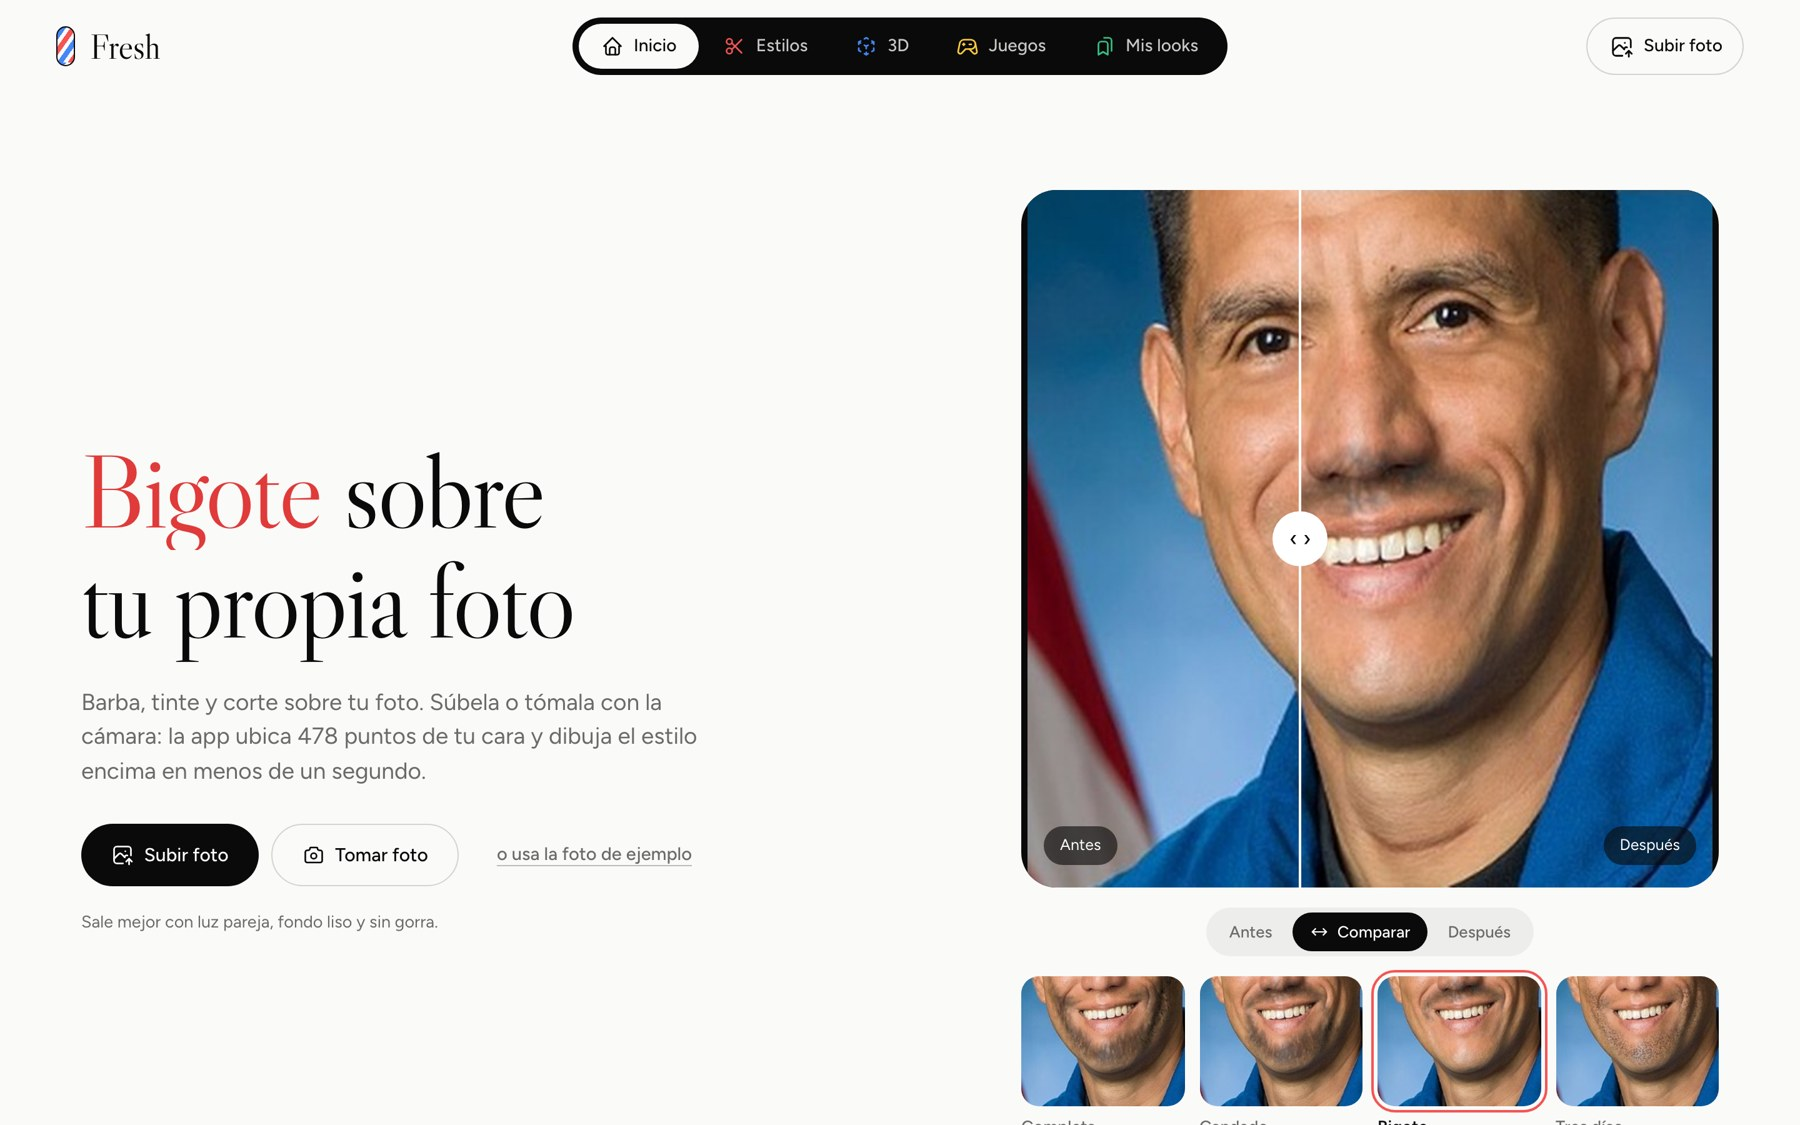
\includegraphics[width=\linewidth]{ui_inicio.jpg}
    \end{column}
  \end{columns}
\end{frame}

\begin{frame}{Qué hace Fresh}
  \begin{columns}[T]
    \begin{column}{0.24\textwidth}
      \tono{red}{\textbf{Estilos}}\\[0.2em]
      \small Barba, tinte (también en la barba), 8 cortes, en vivo con la cámara.
    \end{column}
    \begin{column}{0.24\textwidth}
      \tono{blue}{\textbf{3D}}\\[0.2em]
      \small Espejo 3D desde una foto, peluca 3D escaneada, avatar en vivo.
    \end{column}
    \begin{column}{0.24\textwidth}
      \tono{yellow}{\textbf{Juegos}}\\[0.2em]
      \small Contrarreloj de afeitado y ``¿cuántas gaussianas eres?''.
    \end{column}
    \begin{column}{0.24\textwidth}
      \tono{green}{\textbf{Mis looks}}\\[0.2em]
      \small Combinar estilos, guardar y ficha para el barbero.
    \end{column}
  \end{columns}
  \vspace{1em}
  \centering
  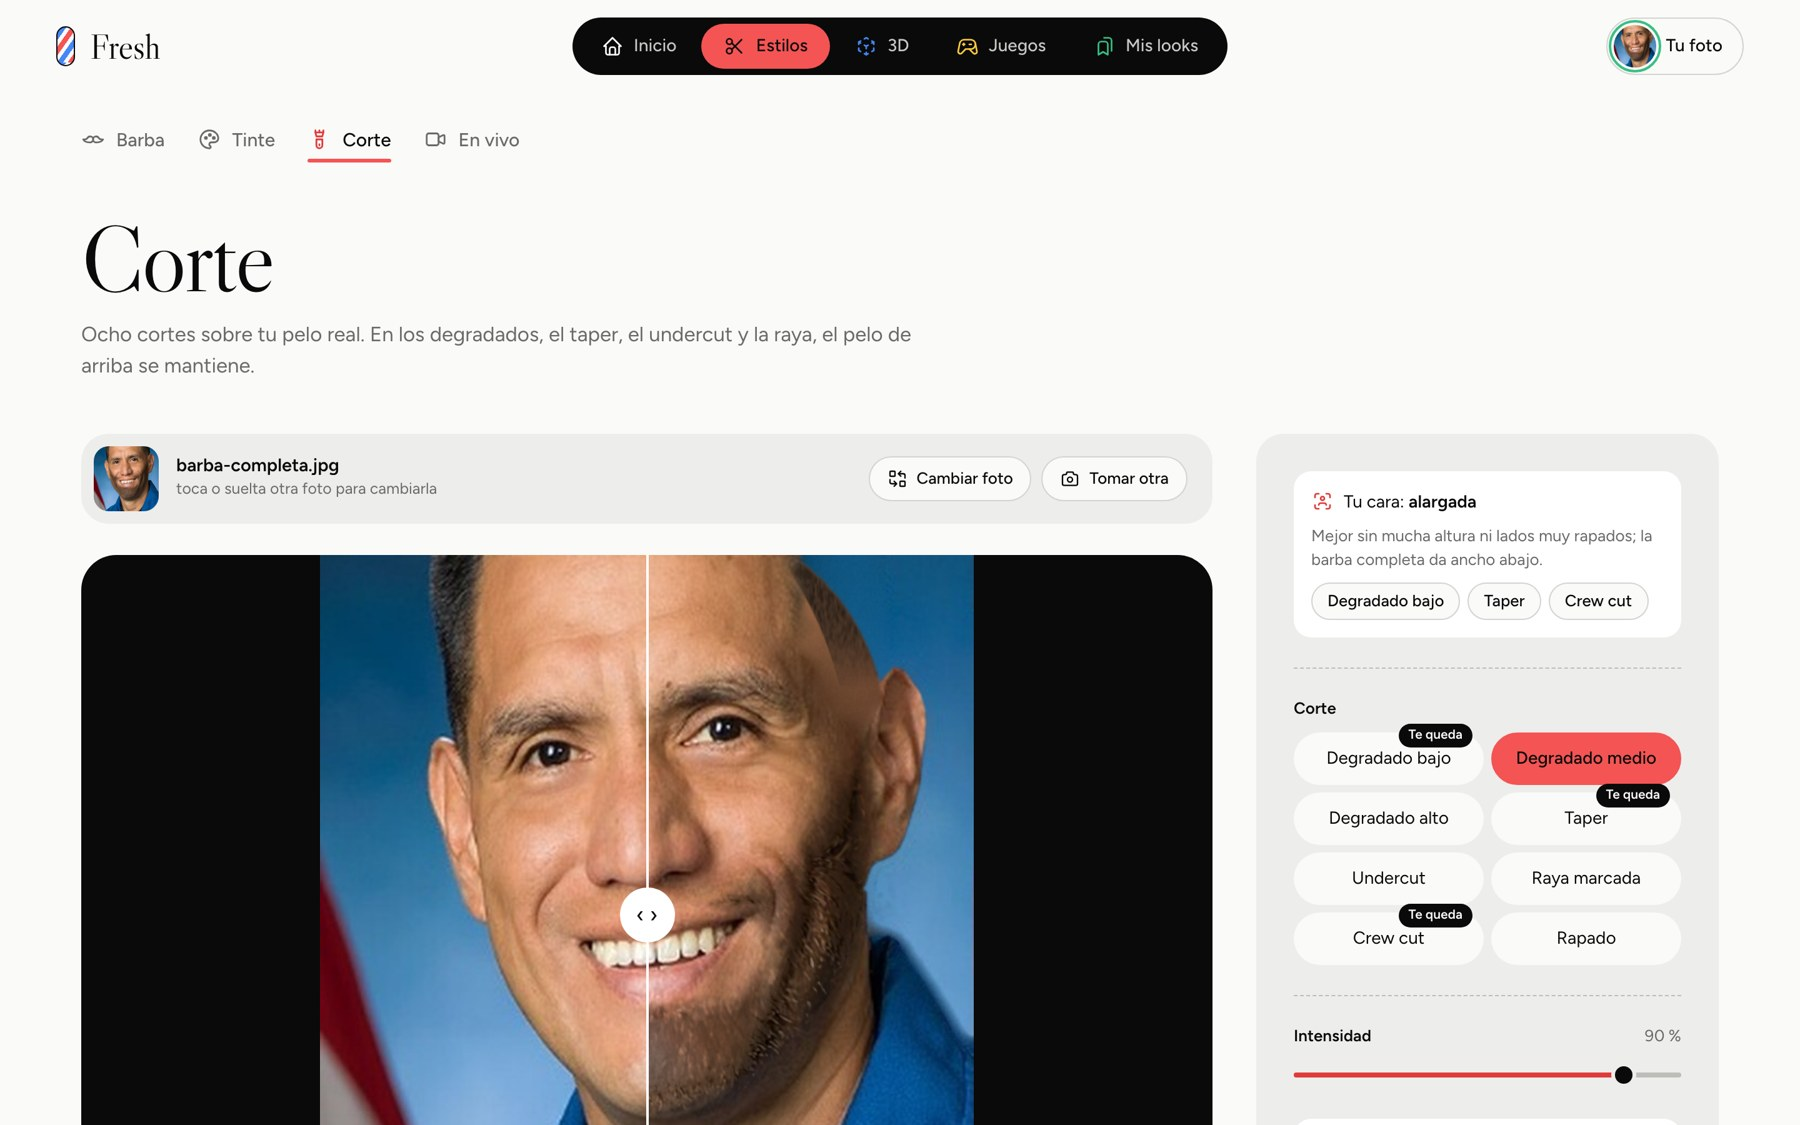
\includegraphics[width=0.5\linewidth]{ui_corte.jpg}
\end{frame}

\begin{frame}{Arquitectura}
  \centering
  \vfill
  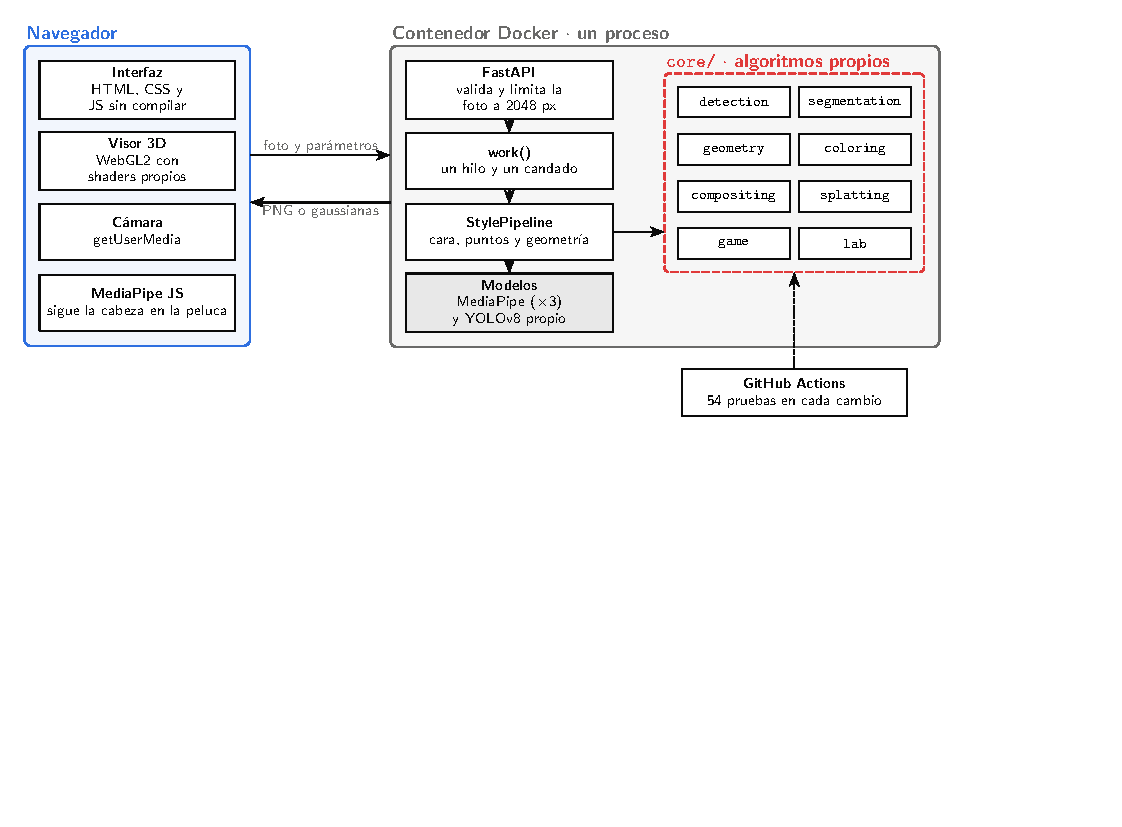
\includegraphics[width=0.96\linewidth]{diagrama_arquitectura.pdf}
  \vfill
  \nota{Un solo proceso sirve la interfaz y la API; cada llamada al pipeline corre en un hilo con candado. Se levanta con \texttt{docker compose up}.}
\end{frame}

\begin{frame}{Qué es nuestro y qué no}
  \begin{columns}[T]
    \begin{column}{0.46\textwidth}
      \textbf{De librerías o modelos}
      \begin{itemize}
        \item 478 puntos de la cara (MediaPipe)
        \item Segmentación base del pelo (MediaPipe)
        \item Puntos de la mano (MediaPipe)
        \item Arquitectura YOLOv8 (Ultralytics)
      \end{itemize}
    \end{column}
    \begin{column}{0.50\textwidth}
      \textbf{Implementado por el equipo}
      \begin{itemize}
        \item Delaunay (Fortune), warp afín, bilineal
        \item Composición de barba y tinte en CIELAB
        \item Motor de 8 cortes con relleno pull-push
        \item Física de hebras (Verlet + PBD)
        \item Gaussianas 2D y 3D, visor WebGL2, \texttt{.ply}
        \item Peluca 3D multivista
        \item Ajuste fino de YOLO para pelo (mAP50 0{,}968)
      \end{itemize}
    \end{column}
  \end{columns}
\end{frame}

\begin{frame}{El pipeline completo}
  \centering
  \vfill
  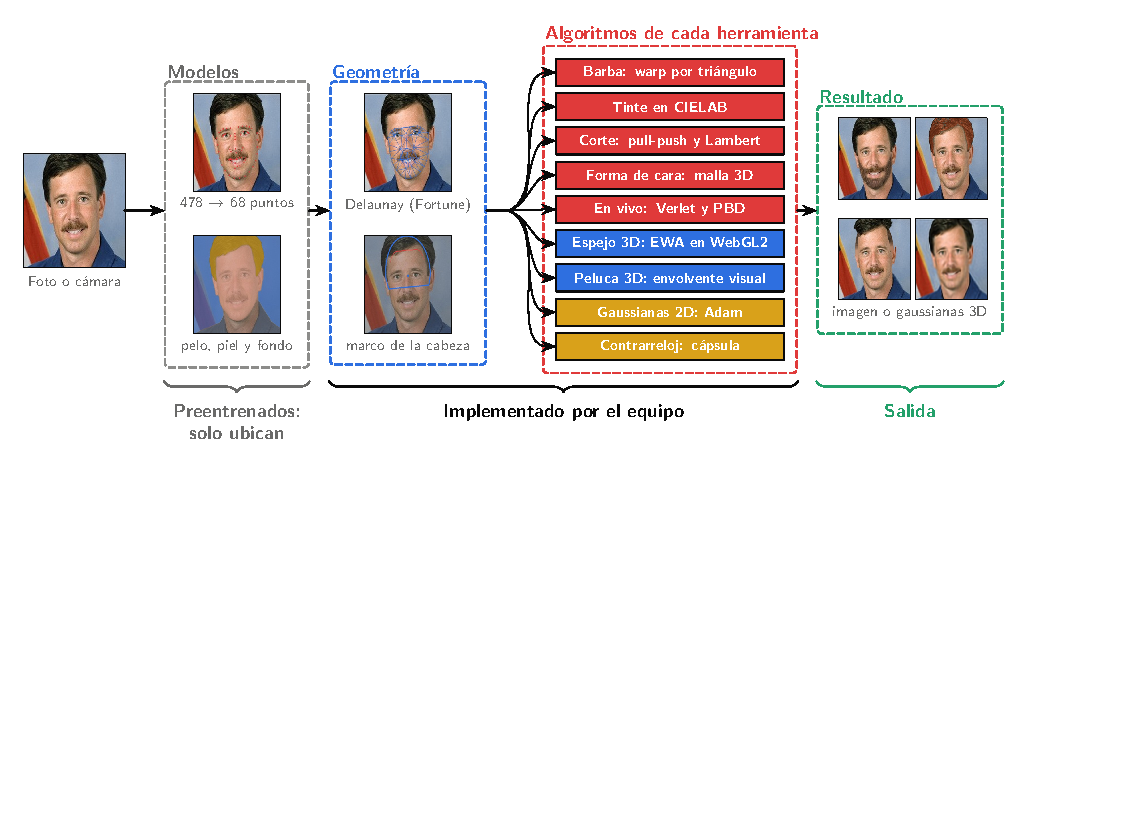
\includegraphics[width=\linewidth]{diagrama_general.pdf}
  \vfill
  \nota{En gris, lo que viene de modelos preentrenados. Todo lo demás lo escribió el equipo.}
\end{frame}

\begin{frame}{Temas del curso que aplicamos}
  \small
  \begin{columns}[T]
    \begin{column}{0.48\textwidth}
      \textbf{6.1 Imágenes}
      \begin{itemize}
        \item Color: tinte en CIELAB, barba en YCrCb
        \item Muestreo: pirámide pull-push
        \item Interpolación: bilineal y baricéntricas
      \end{itemize}
      \textbf{6.2 Geometría computacional}
      \begin{itemize}
        \item Línea de barrido: Fortune
        \item Voronoi y Delaunay, casco convexo
      \end{itemize}
    \end{column}
    \begin{column}{0.48\textwidth}
      \textbf{6.3 Sistemas 3D}
      \begin{itemize}
        \item Shaders propios en WebGL2
        \item Rasterización por baricéntricas
        \item Lambert y mapeo de texturas
        \item Algoritmo del pintor (counting sort)
        \item Gaussian Splatting con proyección EWA
      \end{itemize}
      \textbf{6.4 Visión}
      \begin{itemize}
        \item Tensor de estructura; YOLO con ajuste fino
      \end{itemize}
    \end{column}
  \end{columns}
  \vspace{0.6em}
  \nota{Los modelos solo ubican la cara, el pelo y la mano. Cerca del 87~\% del núcleo es gráfica propia.}
\end{frame}

\begin{frame}{De puntos a malla: Delaunay con Fortune}
  \small
  \begin{columns}[T]
    \begin{column}{0.55\textwidth}
      \begin{itemize}
        \item 478 puntos $\rightarrow$ 68 (iBUG) $+$ 15 bajo el mentón.
        \item Delaunay: círculos circunscritos vacíos; evita triángulos ``aguja''.
        \item \textbf{Fortune}: línea de barrido y \emph{beach line} de parábolas.
        \begin{itemize}
          \item evento de sitio: aparece un arco;
          \item evento de círculo: desaparece un arco $\Rightarrow$ \textbf{un triángulo}.
        \end{itemize}
        \item $O(n\log n)$ con un árbol; la nuestra usa una lista: $O(n^2)$, 3~ms con 83 puntos.
        \item Contra Bowyer--Watson: halla un triángulo del borde que ese método pierde.
        \item Grilla: perturbación mínima y sin triángulos de área cero.
      \end{itemize}
    \end{column}
    \begin{column}{0.38\textwidth}
      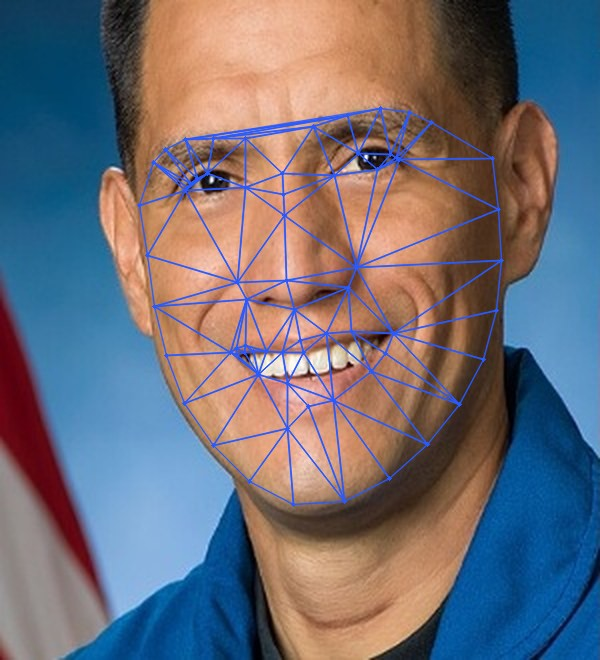
\includegraphics[width=\linewidth]{malla.jpg}
    \end{column}
  \end{columns}
\end{frame}

\begin{frame}{Barba: el proceso}
  \centering
  \vfill
  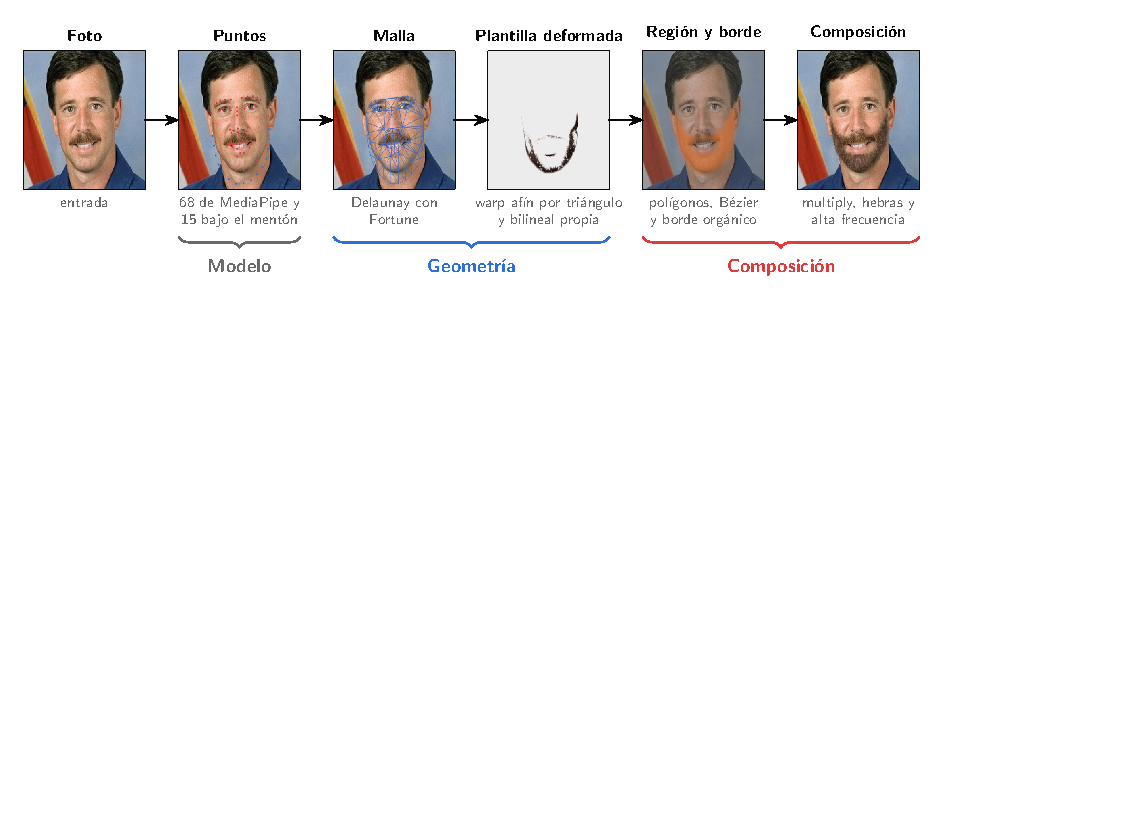
\includegraphics[width=\linewidth]{diagrama_barba.pdf}
  \vfill
  \nota{La misma triangulación en la plantilla y en la cara: cada triángulo tiene su propia transformación afín.}
\end{frame}

\begin{frame}{Barba con plantillas reales}
  \begin{itemize}
    \item 10 barbas reales de CelebAMask-HQ, cada una con sus 83 puntos.
    \item Warp afín por triángulo: afín inversa $3\times3$, prueba baricéntrica $\lambda_i\ge0$, muestreo bilineal propio.
    \item Tres capas: \emph{multiply} (la piel sigue viéndose), hebras con Bézier y detalle de alta frecuencia.
  \end{itemize}
  \vspace{0.6em}
  \centering
  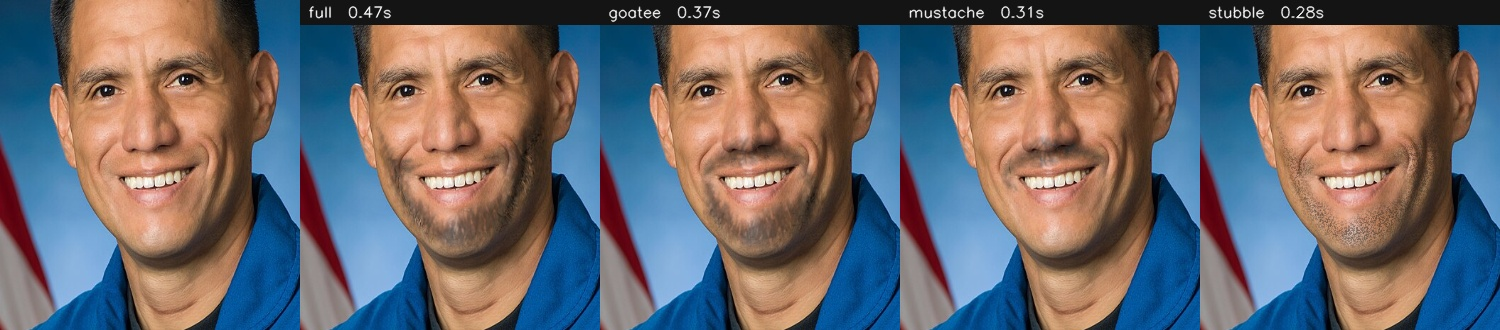
\includegraphics[width=0.92\linewidth]{barba_estilos.jpg}
\end{frame}

\begin{frame}{Tinte: el proceso}
  \centering
  \vfill
  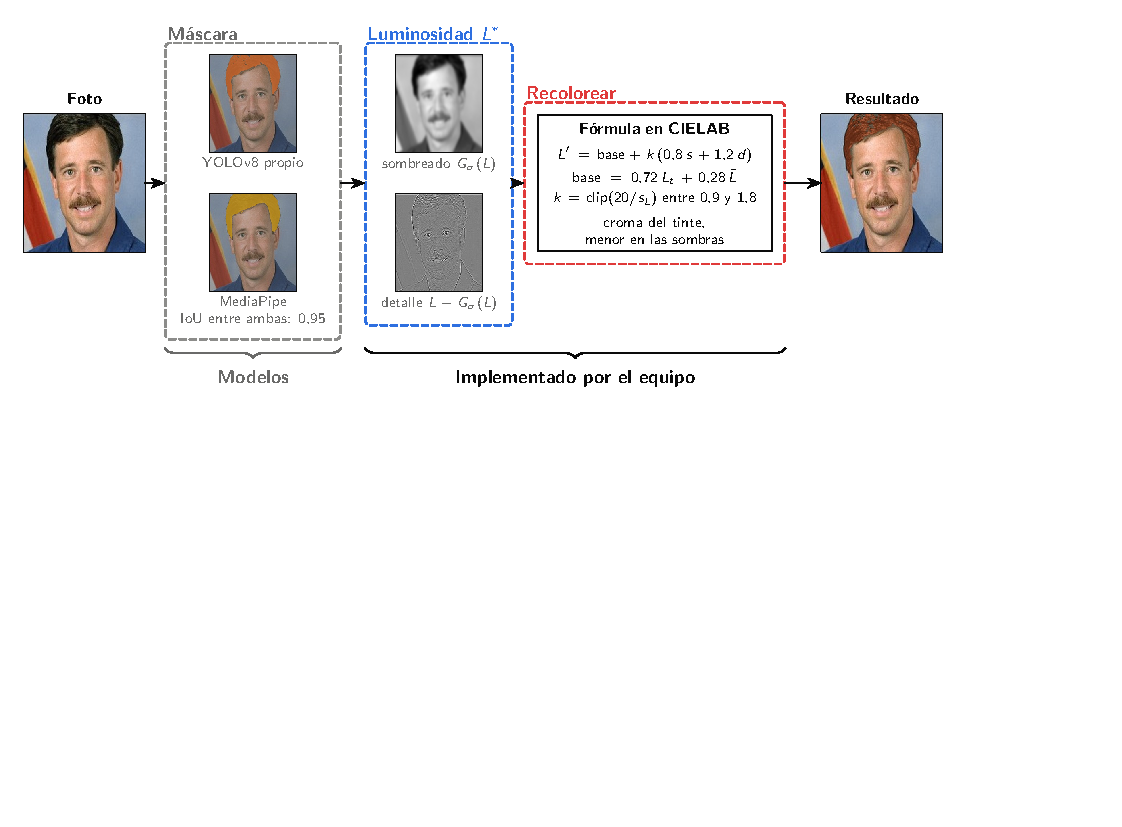
\includegraphics[width=\linewidth]{diagrama_tinte.pdf}
  \vfill
  \nota{En CIELAB el brillo y el color van separados; por eso un pelo negro puede quedar rubio.}
\end{frame}

\begin{frame}{Tinte en CIELAB}
  \begin{columns}[T]
    \begin{column}{0.44\textwidth}
      \begin{itemize}
        \item La luminosidad base va hacia el tinte; el detalle de cada mechón se conserva:
      \end{itemize}
      {\small
      \begin{align*}
        L' &= \underbrace{0{,}72L_t+0{,}28\bar L}_{\text{base}}\\
           &\quad + k\,(0{,}8\,\text{sombra}+1{,}2\,\text{detalle})
      \end{align*}}
      \begin{itemize}
        \item El croma baja en las sombras, como un pigmento real.
        \item Máscara: MediaPipe o \textbf{nuestro YOLO}; la app muestra la IoU entre los dos.
      \end{itemize}
    \end{column}
    \begin{column}{0.54\textwidth}
      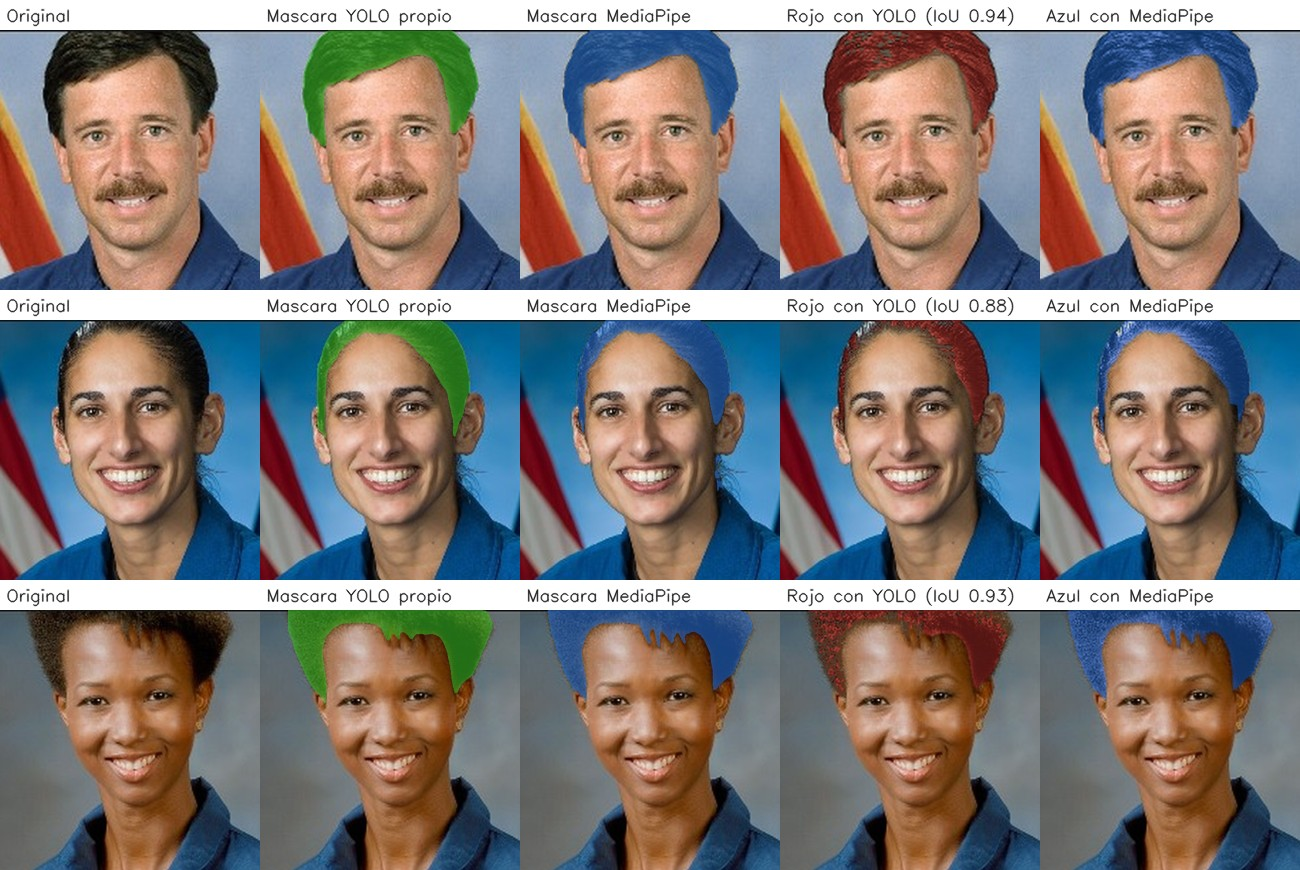
\includegraphics[width=\linewidth]{tinte_modelos.jpg}
    \end{column}
  \end{columns}
\end{frame}

\begin{frame}{Corte: el proceso}
  \centering
  \vfill
  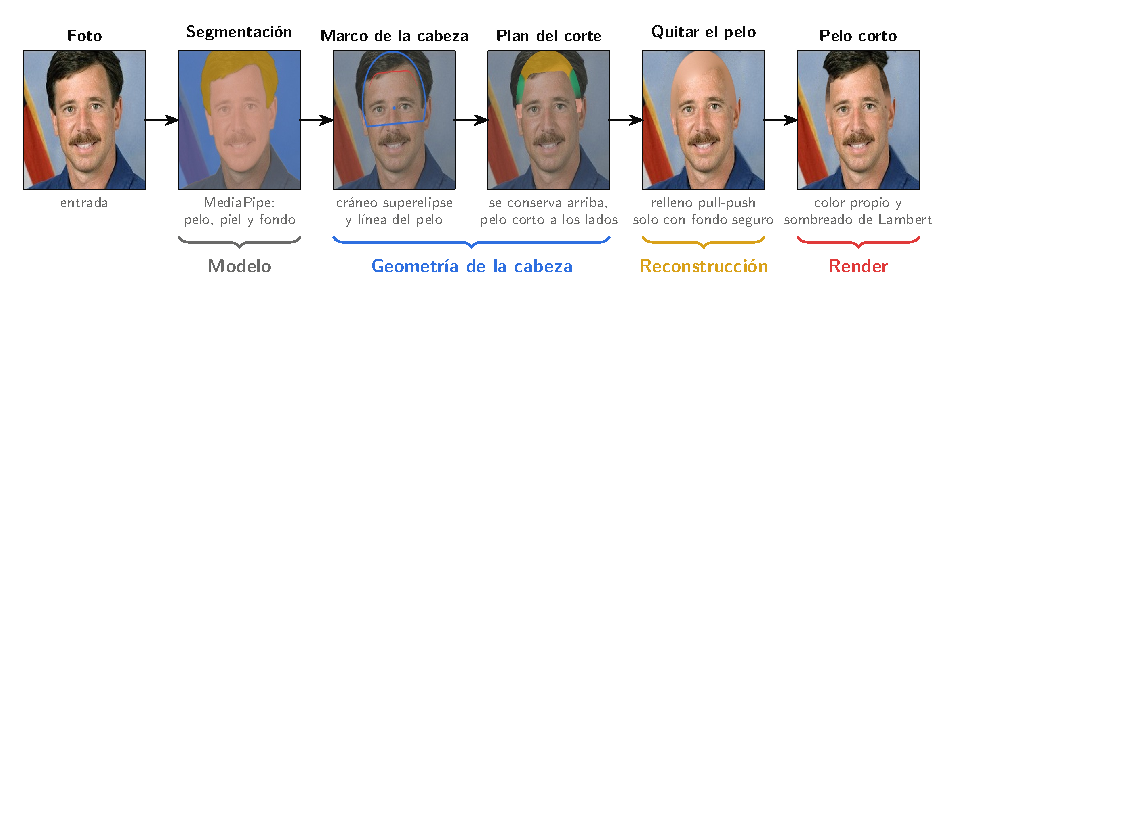
\includegraphics[width=\linewidth]{diagrama_corte.pdf}
  \vfill
  \nota{Todo se mide en anchos de cabeza, así los mismos parámetros sirven para cualquier foto.}
\end{frame}

\begin{frame}{Cortar el pelo: primero hay que quitarlo}
  \begin{itemize}
    \item El pelo que sobra deja un hueco: ¿qué había detrás?
    \item Telea toma color de todo el borde, \textbf{incluido el pelo} $\Rightarrow$ pelo fantasma.
    \item \textbf{Pull-push} con fuentes elegidas: solo píxeles de fondo seguro.
  \end{itemize}
  \vspace{0.5em}
  \centering
  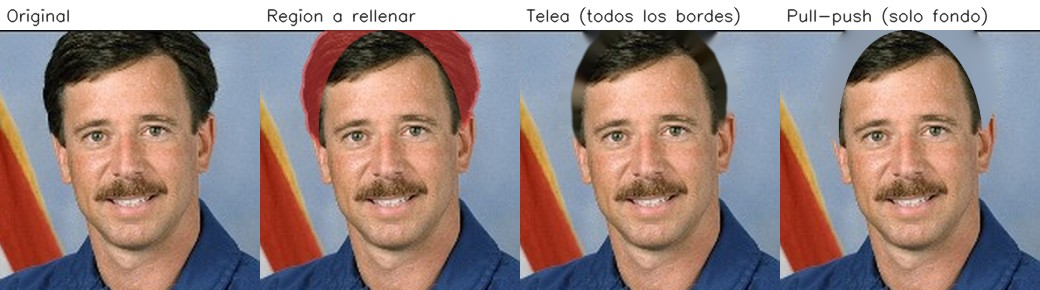
\includegraphics[width=0.9\linewidth]{pull_push.jpg}
  \nota{Después: se borran mechones sueltos y el relleno recibe la textura local del fondo.}
\end{frame}

\begin{frame}{Ocho cortes sobre el mismo marco de la cabeza}
  \begin{columns}[T]
    \begin{column}{0.48\textwidth}
      \begin{itemize}
        \item Marco en anchos de cabeza: igual para 600 o 4000~px.
        \item Cráneo: superelipse ajustada a la coronilla.
      \end{itemize}
    \end{column}
    \begin{column}{0.48\textwidth}
      \begin{itemize}
        \item Línea del pelo desde la frente visible.
        \item Pelo corto del color propio, sombreado de Lambert.
      \end{itemize}
    \end{column}
  \end{columns}
  \vspace{0.2em}
  \centering
  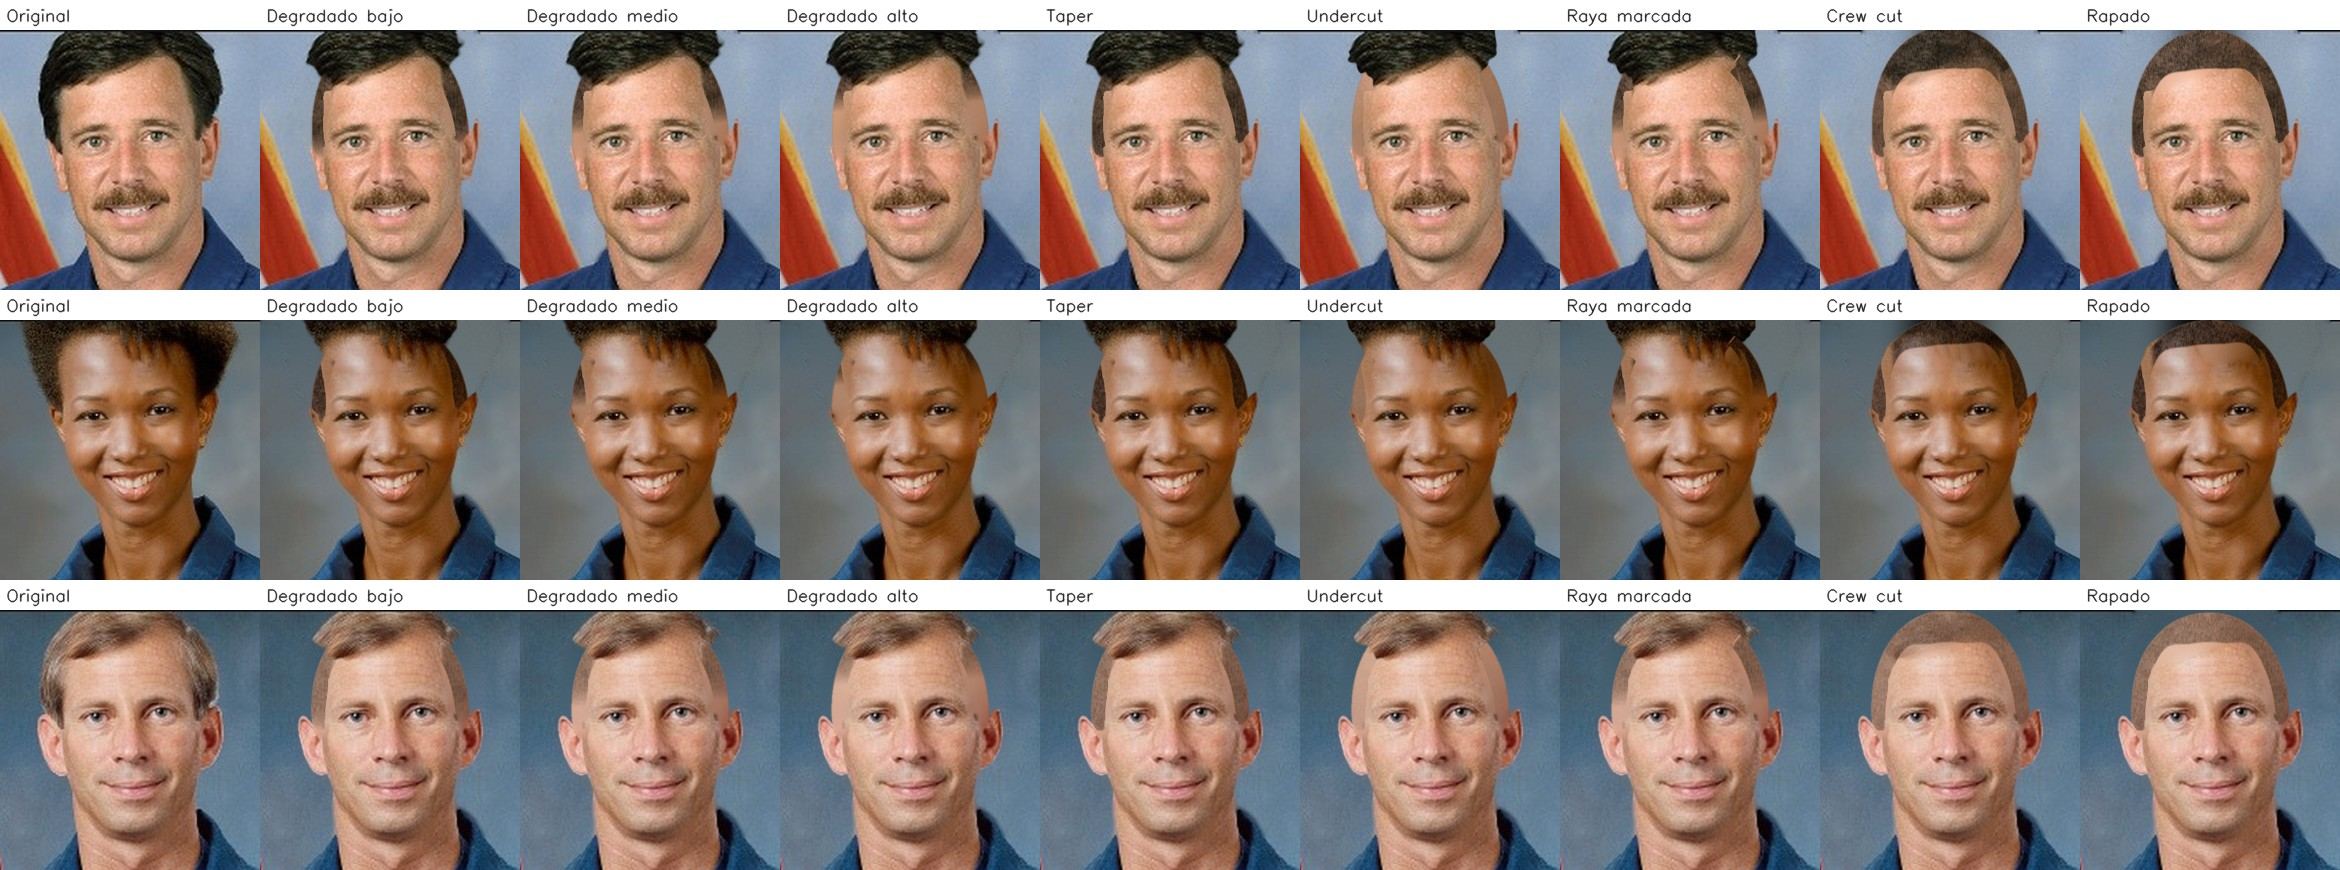
\includegraphics[width=0.95\linewidth]{cortes.jpg}
\end{frame}

\begin{frame}{Combinar y llevárselo al barbero}
  \begin{columns}[T]
    \begin{column}{0.6\textwidth}
      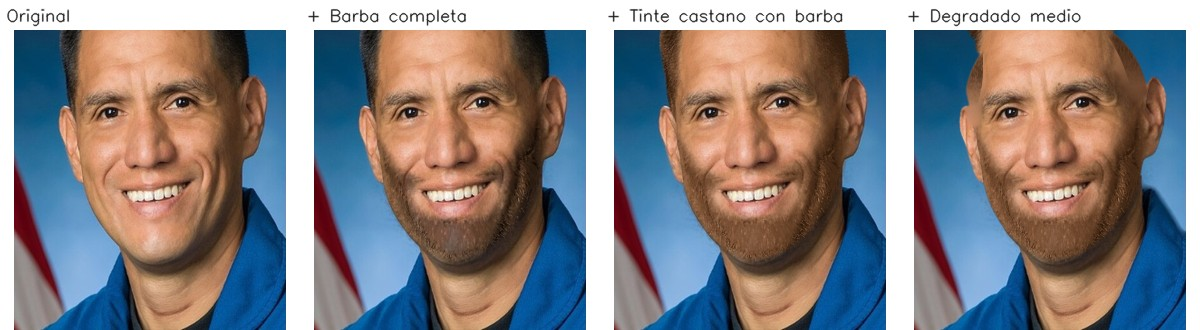
\includegraphics[width=\linewidth]{combinado.jpg}
      \vspace{0.4em}
      \begin{itemize}
        \item Cada resultado pasa a ser la foto de la herramienta siguiente.
        \item Barba en el tinte: textura, color y tensor de estructura (descarta el borde de la mandíbula).
      \end{itemize}
    \end{column}
    \begin{column}{0.36\textwidth}
      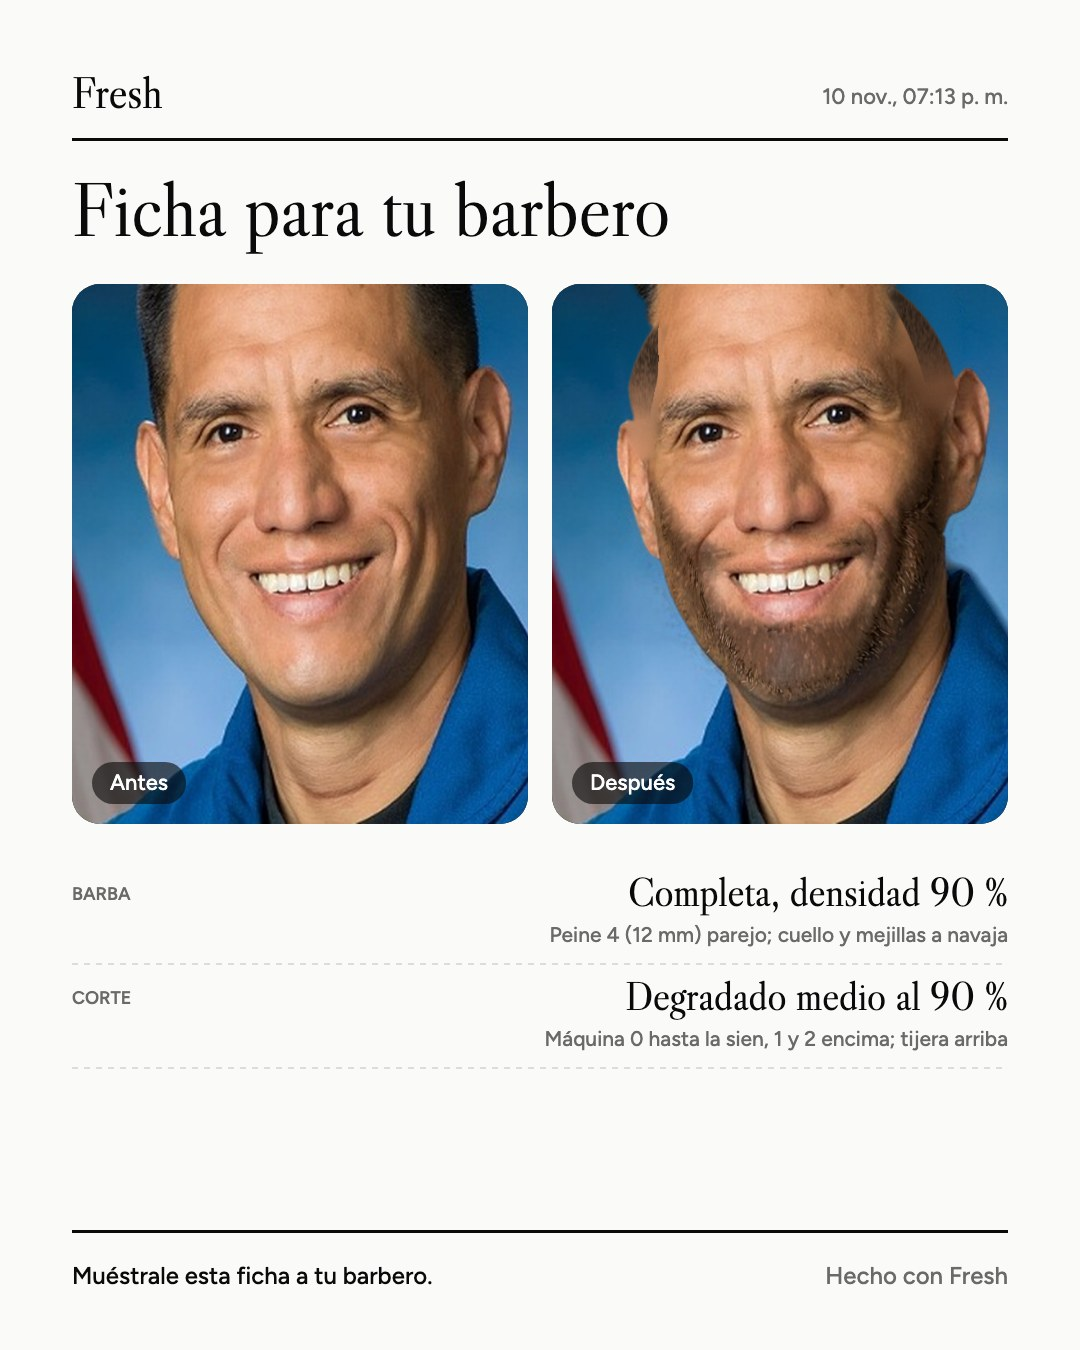
\includegraphics[width=\linewidth]{ui_ficha.jpg}
    \end{column}
  \end{columns}
\end{frame}

\begin{frame}{¿Qué te queda? Forma de la cara}
  \begin{columns}[T]
    \begin{column}{0.55\textwidth}
      \begin{itemize}
        \item Medidas sobre la malla 3D, divididas por el ancho de pómulos.
        \item Las caras varían poco $\Rightarrow$ umbrales en desviaciones $z$, calibrados con \textbf{419 caras}.
        \item Ovalada, redonda, cuadrada, alargada o corazón.
        \item Cada forma sugiere cortes y barbas, marcados en la interfaz.
      \end{itemize}
      \nota{Es una heurística, no una regla estética.}
    \end{column}
    \begin{column}{0.36\textwidth}
      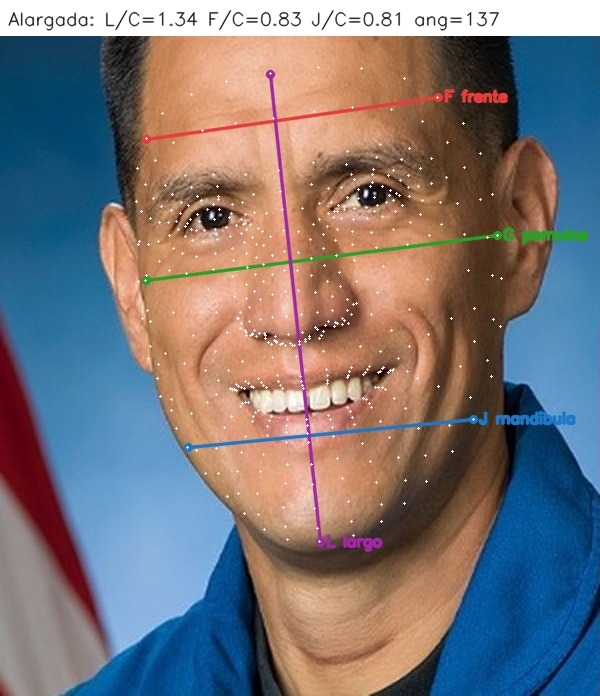
\includegraphics[width=\linewidth]{forma_cara.jpg}
    \end{column}
  \end{columns}
\end{frame}

\begin{frame}{En vivo: el proceso}
  \centering
  \vfill
  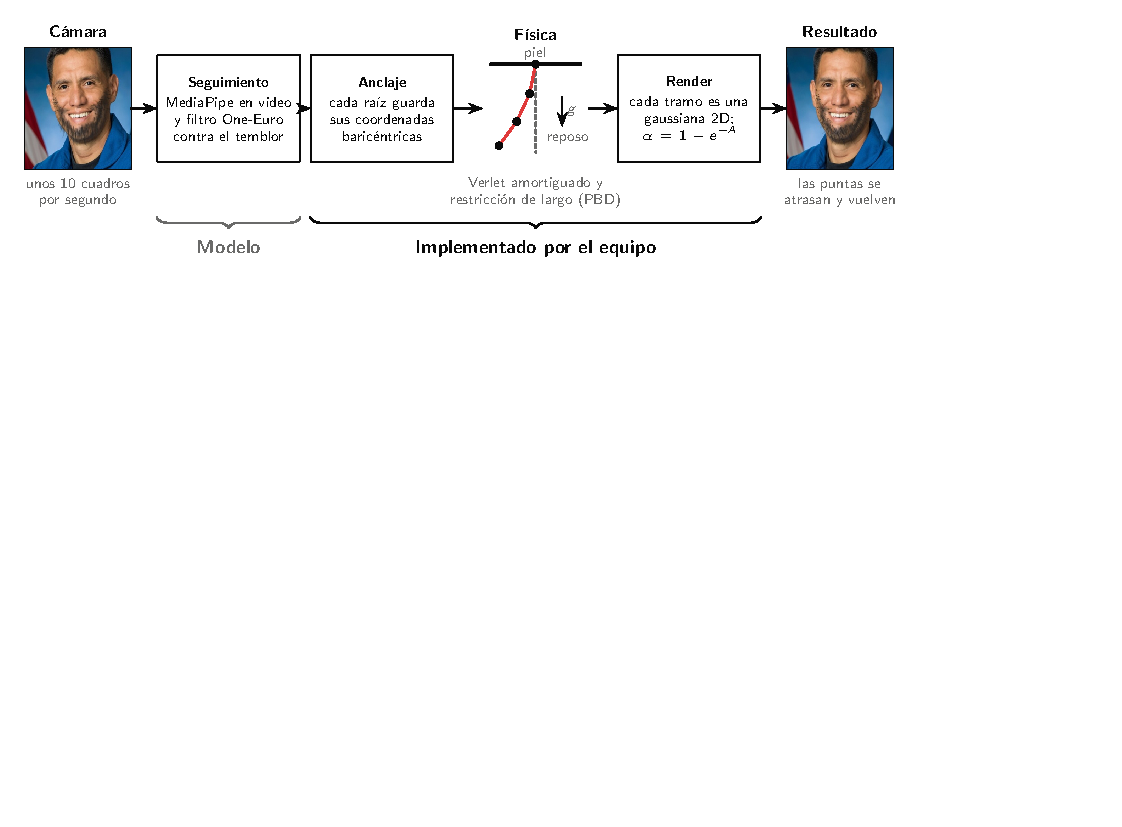
\includegraphics[width=\linewidth]{diagrama_vivo.pdf}
  \vfill
  \nota{Las raíces siguen la piel con coordenadas baricéntricas; Verlet y PBD mueven las puntas.}
\end{frame}

\begin{frame}{Barba con física}
  \begin{columns}[T]
    \begin{column}{0.48\textwidth}
      \begin{itemize}
        \item Cada pelo: 4 partículas; la raíz, en coordenadas baricéntricas de la malla.
        \item Verlet amortiguado, resorte a la pose de reposo y restricción de distancia (PBD).
      \end{itemize}
      \[
        x \leftarrow x + 0{,}86\,(x-x_{\text{prev}}) + g\,h^2
      \]
      \begin{itemize}
        \item Cada tramo se dibuja como una gaussiana alargada: $\alpha=1-e^{-\sum o_iG_i}$.
      \end{itemize}
    \end{column}
    \begin{column}{0.48\textwidth}
      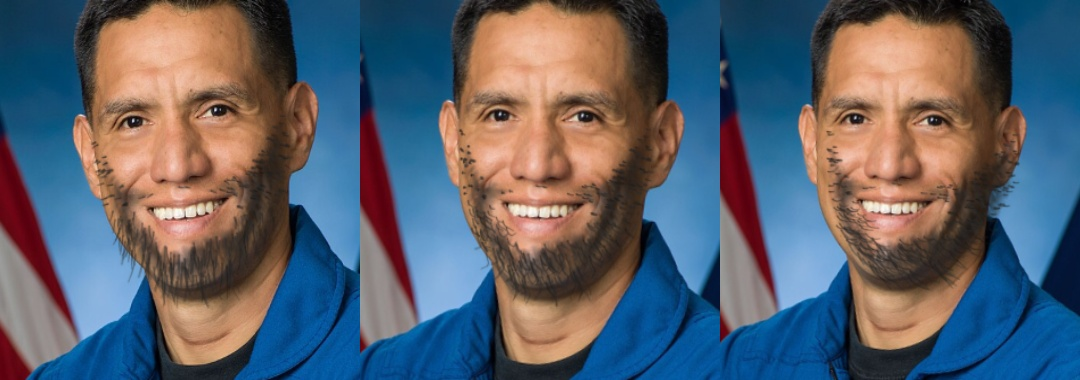
\includegraphics[width=\linewidth]{fisica.jpg}
    \end{column}
  \end{columns}
\end{frame}

\begin{frame}{Gaussianas 2D: el proceso}
  \centering
  \vfill
  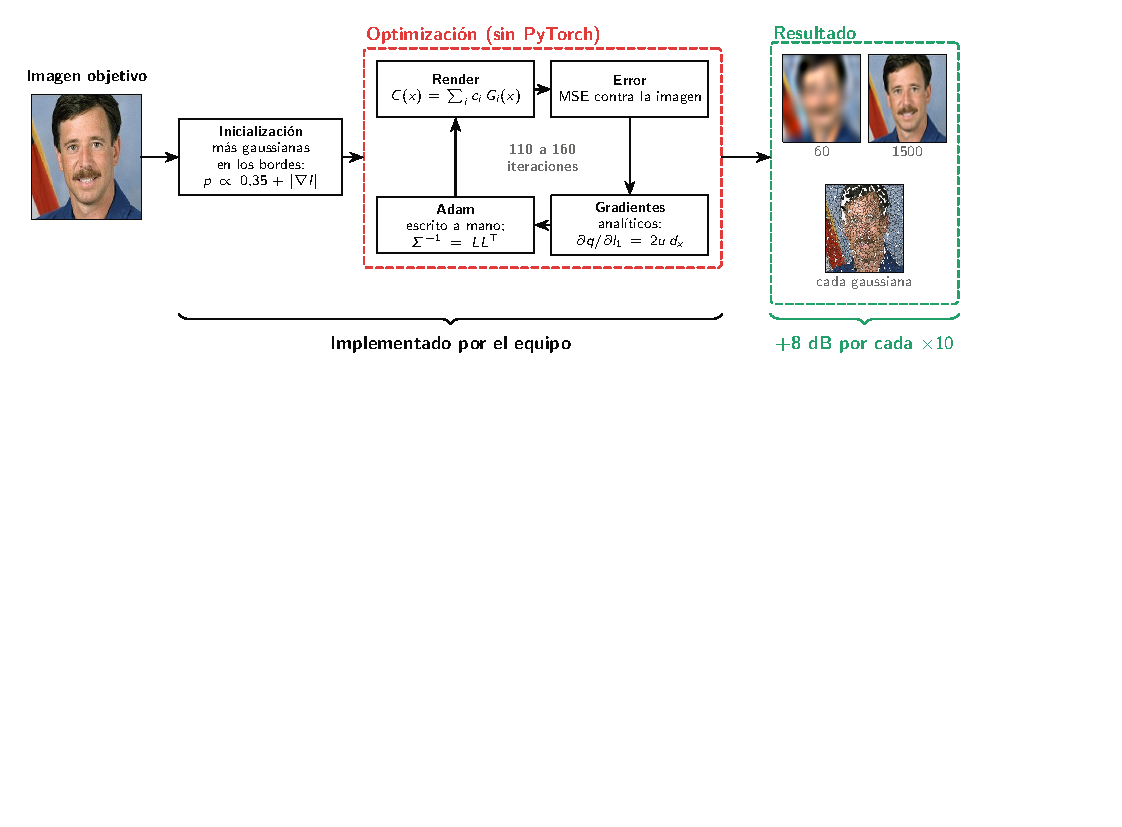
\includegraphics[width=\linewidth]{diagrama_gaussianas.pdf}
  \vfill
  \nota{Los gradientes y Adam están escritos a mano, sin PyTorch.}
\end{frame}

\begin{frame}{¿Cuántas gaussianas eres?}
  \begin{itemize}
    \item Un retrato hecho solo de $N$ gaussianas 2D, ajustadas con gradientes analíticos y Adam escrito a mano.
    \item El PSNR sube unos 8~dB cada vez que $N$ se multiplica por 10.
  \end{itemize}
  \vspace{0.4em}
  \centering
  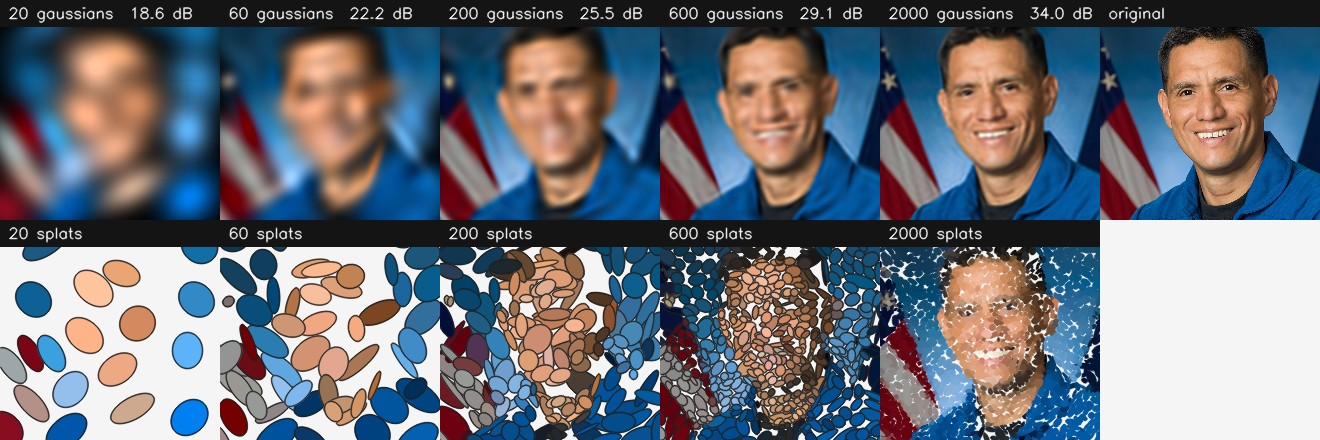
\includegraphics[width=0.9\linewidth]{gaussianas2d.jpg}
\end{frame}

\begin{frame}{Espejo 3D: el proceso}
  \centering
  \vfill
  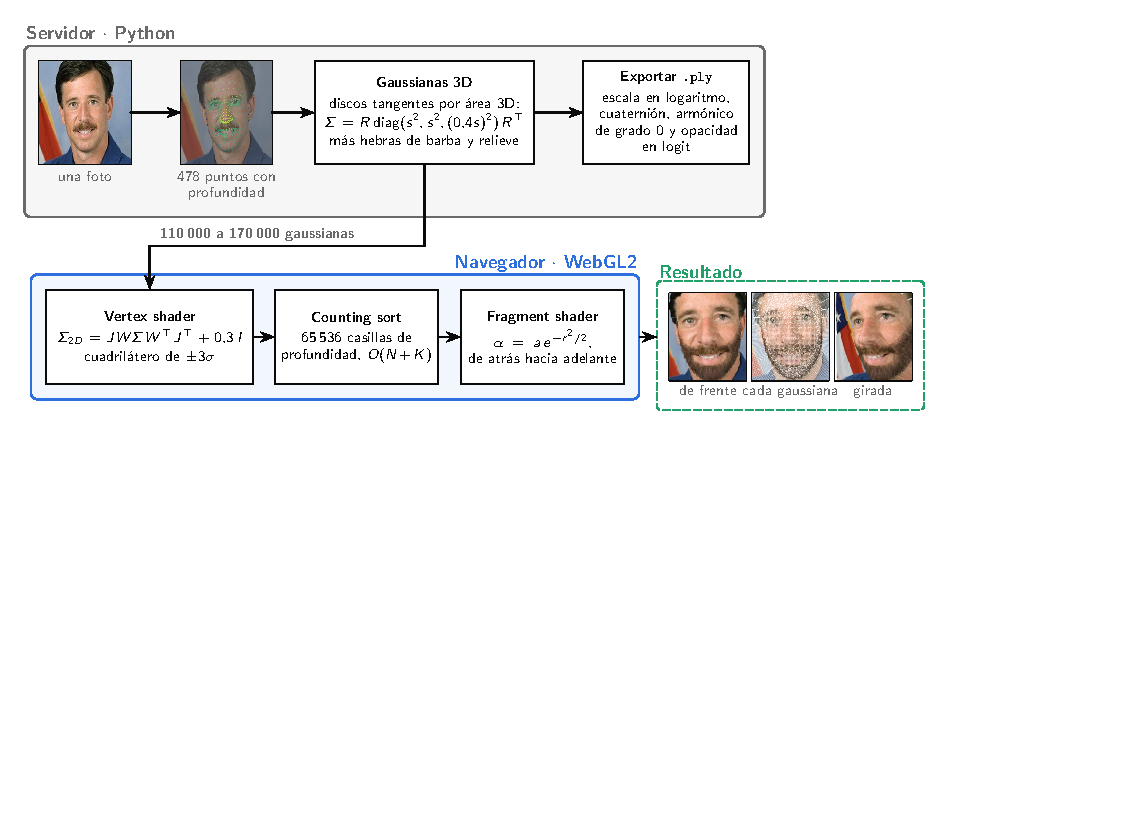
\includegraphics[width=\linewidth]{diagrama_espejo.pdf}
  \vfill
  \nota{El servidor arma las gaussianas; la GPU del navegador las proyecta, ordena y mezcla.}
\end{frame}

\begin{frame}{Espejo 3D: Gaussian Splatting en WebGL2}
  \begin{columns}[T]
    \begin{column}{0.4\textwidth}
      \begin{itemize}
        \item Una foto + malla 3D $\rightarrow$ 110\,000 a 170\,000 gaussianas.
        \item Proyección EWA:
      \end{itemize}
      \[ \Sigma_{2D} = J\,W\,\Sigma\,W^\top J^\top \]
      \begin{itemize}
        \item Counting sort de atrás hacia adelante, mezcla alfa.
        \item Exporta \texttt{.ply} estándar de 3DGS.
      \end{itemize}
    \end{column}
    \begin{column}{0.58\textwidth}
      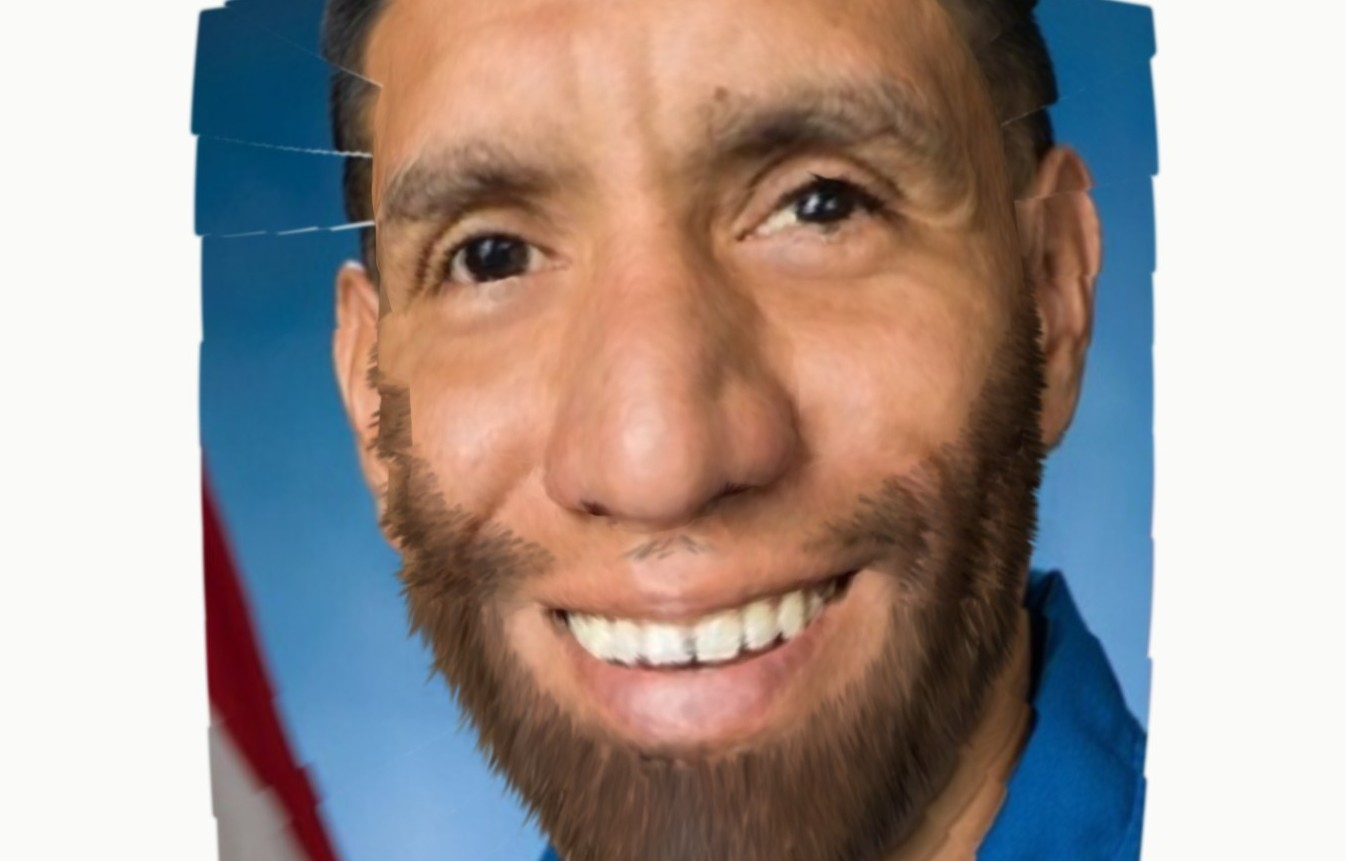
\includegraphics[width=0.49\linewidth]{espejo3d_frente.jpg}\hfill
      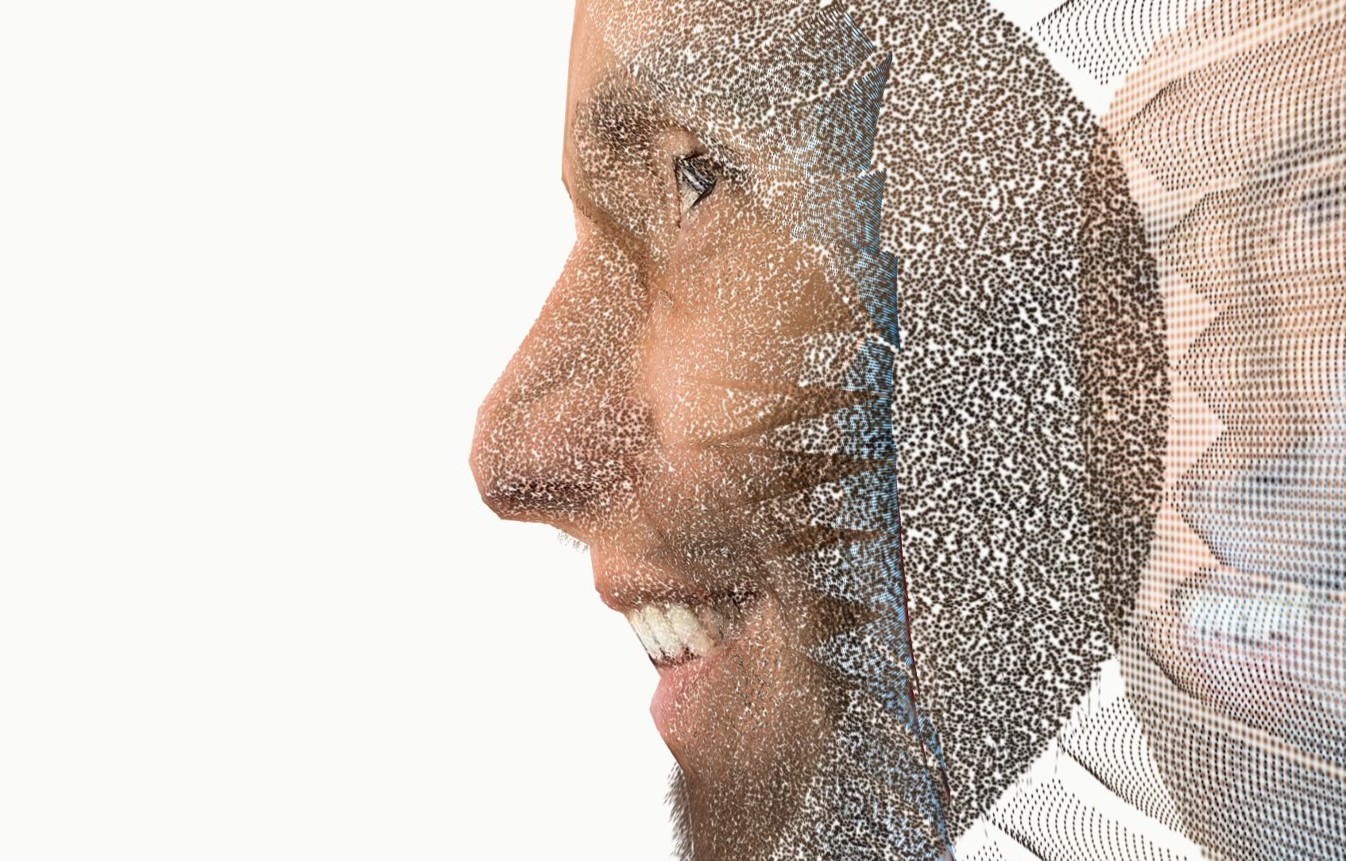
\includegraphics[width=0.49\linewidth]{espejo3d_splats.jpg}
      \nota{Una sola vista: sin nuca; al girar mucho, el relieve se estira.}
    \end{column}
  \end{columns}
\end{frame}

\begin{frame}{Peluca 3D: el proceso}
  \centering
  \vfill
  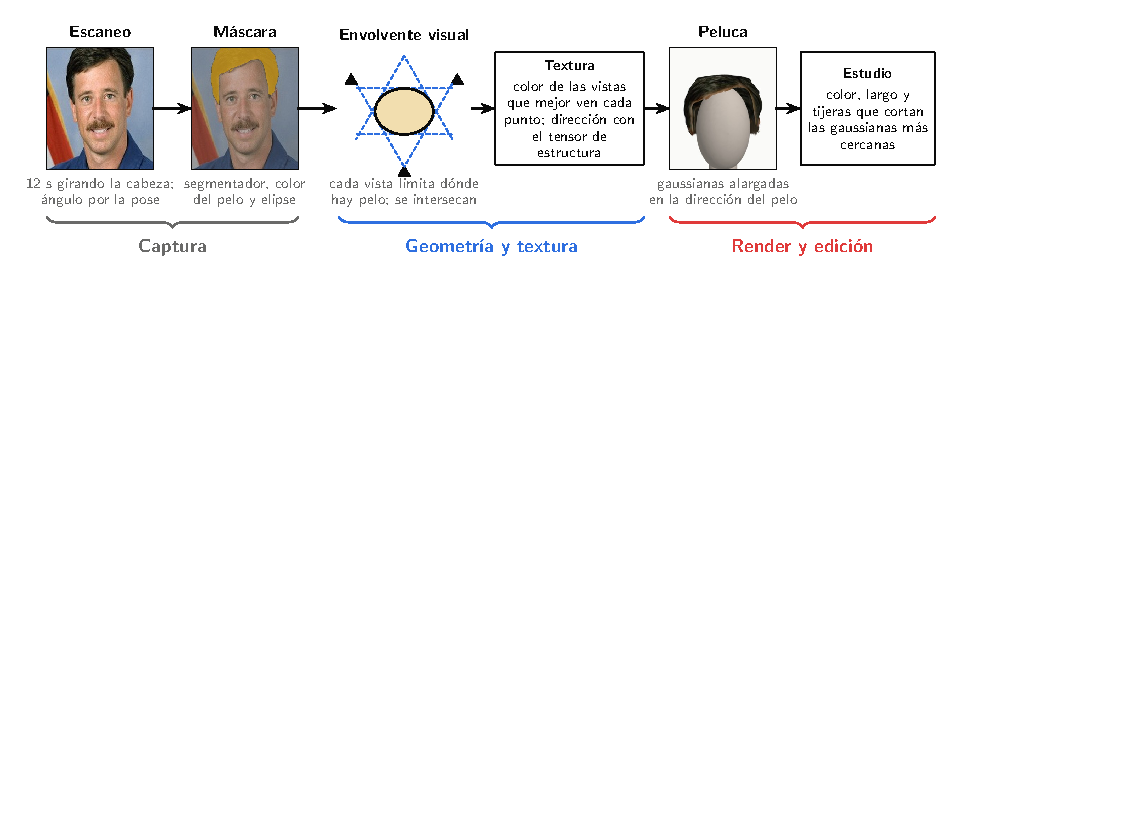
\includegraphics[width=\linewidth]{diagrama_peluca.pdf}
  \vfill
  \nota{Cada vista acota dónde puede haber pelo; la intersección es la forma de la peluca.}
\end{frame}

\begin{frame}{Peluca 3D}
  \begin{columns}[T]
    \begin{column}{0.52\textwidth}
      \begin{itemize}
        \item Escaneo de 12~s girando la cabeza 180°.
        \item \emph{Visual hull} por cortes: cada vista limita dónde hay pelo en cada altura y dirección.
        \item Textura de las vistas que mejor ven cada punto; la nuca, del último pelo de cada perfil.
        \item Estudio: color, largo y tijeras sobre las gaussianas.
      \end{itemize}
    \end{column}
    \begin{column}{0.42\textwidth}
      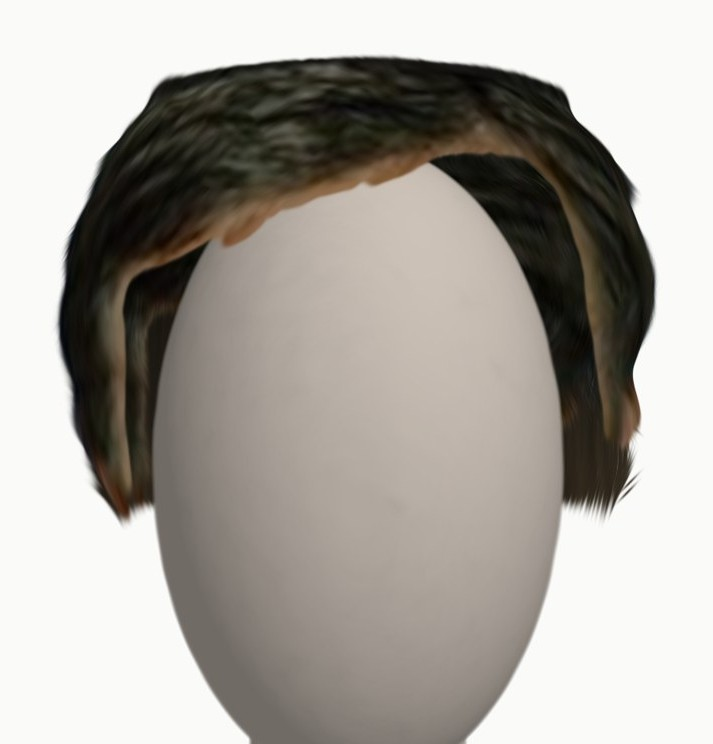
\includegraphics[width=\linewidth]{peluca3d.jpg}
    \end{column}
  \end{columns}
\end{frame}

\begin{frame}{Contrarreloj: el proceso}
  \centering
  \vfill
  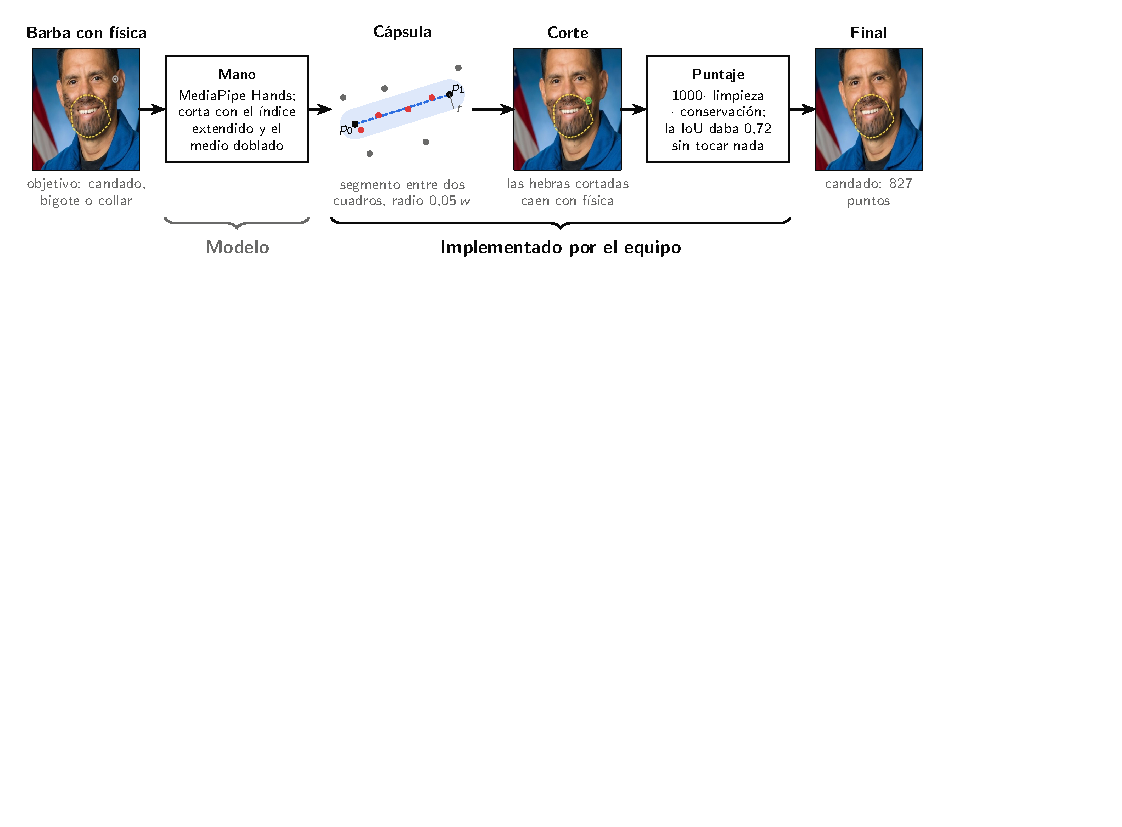
\includegraphics[width=\linewidth]{diagrama_juego.pdf}
  \vfill
  \nota{A 10 cuadros por segundo el dedo salta; la cápsula corta todo lo que quedó en el camino.}
\end{frame}

\begin{frame}{Contrarreloj}
  \begin{itemize}
    \item 30~s para afeitar hasta un estilo objetivo, con el dedo índice o el mouse.
    \item A 10~fps el dedo salta: se corta todo lo que toca la \textbf{cápsula} entre dos cuadros.
    \item Puntaje $=1000\cdot\text{limpieza}\cdot\text{conservación}$; sin tocar nada, 0.
  \end{itemize}
  \vspace{0.5em}
  \centering
  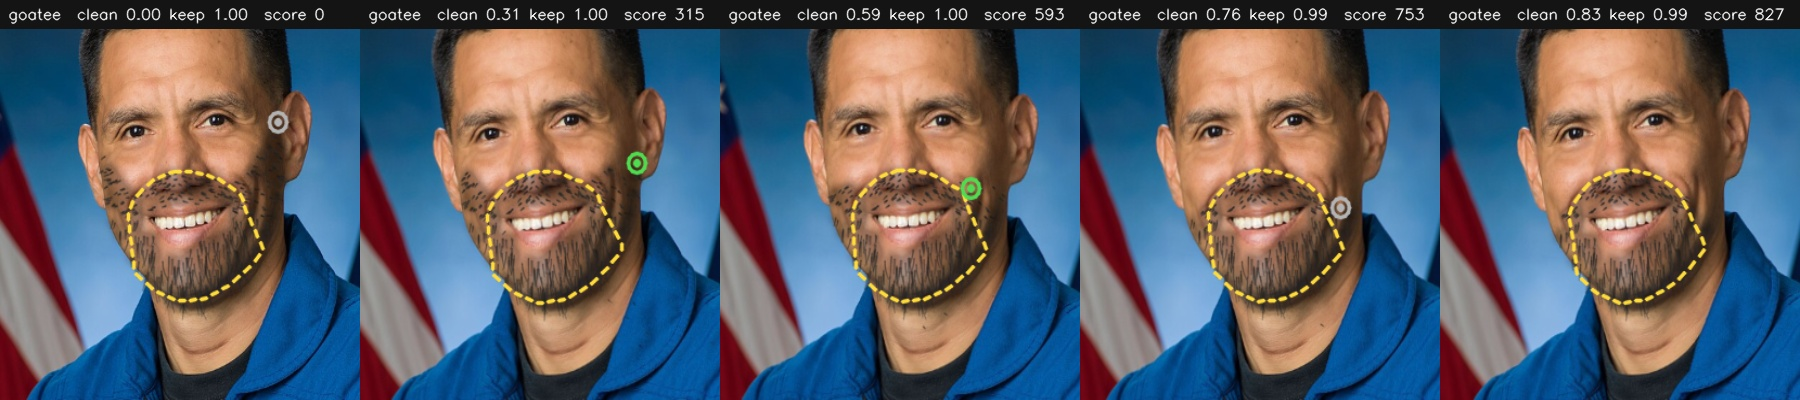
\includegraphics[width=0.92\linewidth]{contrarreloj.jpg}
\end{frame}

\begin{frame}{Calidad y rendimiento}
  \begin{columns}[T]
    \begin{column}{0.46\textwidth}
      \begin{itemize}
        \item 53 pruebas automáticas, integración continua en GitHub Actions.
        \item Docker: un comando, con modelos incluidos.
        \item Probado en 26 caras: piel clara, morena y negra; pelo liso, rizado, largo, corto.
        \item Funciona con o sin YOLO instalado.
      \end{itemize}
    \end{column}
    \begin{column}{0.5\textwidth}
      \small
      \begin{tabularx}{\linewidth}{@{}X r@{}}
        \toprule
        Operación & Tiempo \\
        \midrule
        Corte, foto de celular (Docker) & ${<}\,2$~s \\
        Tinte con YOLO y barba & 2{,}5~s \\
        Espejo 3D, 105\,000 gaussianas & 2{,}6~s \\
        Barba en vivo, por cuadro & 61~ms \\
        Física, por cuadro & 72~ms \\
        \bottomrule
      \end{tabularx}
    \end{column}
  \end{columns}
\end{frame}

\begin{frame}{Límites que conocemos}
  \large
  \begin{itemize}
    \item Sin oclusiones: una mano delante de la cara queda debajo de la barba.
    \item Flequillo sobre un ojo u orejas tapadas: no se inventa el ojo ni la oreja.
    \item Espejo 3D desde una sola vista: sin nuca.
    \item En vivo, unos 10~fps.
  \end{itemize}
  \vspace{0.8em}
  \textbf{Siguiente paso:} tinte en vivo en el navegador con un shader de WebGL.
\end{frame}

\begin{frame}[plain]
  \vfill
  {\usebeamerfont{title}Demo}
  \vspace{1em}

  \Large
  \begin{enumerate}
    \item ¿Cuántas gaussianas eres?
    \item Barba, tinte y corte combinados $\rightarrow$ ficha
    \item En vivo con física
    \item Contrarreloj: ¿quién juega?
    \item Espejo 3D
  \end{enumerate}
  \vfill
\end{frame}

\end{document}
